\section{Strålning genom glas}\label{sec:sunthroughwindowsmethod}


\subsection{Soltimmar under dygnet}
\label{subsec:sunhours}
Under året så varierar antalet soltimmar. Detta kommer av att jordens axel ej är paralell
med jordens rotationsaxel kring solen. I praktiken innebär detta att det är mindre soltimmar
under vinterhalvåret och fler under sommarhalvåret. Då jordens bana kring solen är nästan
cirkulär kan vi approximera antalet soltimmar per dygn som en trigonometrisk funktion.
För Göteborg approximerar vi att årets kortaste dag är $\unit[6]{ timmar}$ och $\unit[32]{minuter}$ och årets längsta
dag är $\unit[17]{ timmar}$ och $\unit[28]{ minuter}$. \cite{sunup} Sedan noterar vi att dagen är som kortast runt den $20$
december.
Detta tillåter oss då att teckna dygnets soltimmar $\tau$ som ekvation \eqref{eq:sunhours}. Här
är $t$ tiden i månader där $t=0$ motsvarar första januari och $t$ är periodiskt över $12$ månader.

\begin{equation}
\label{eq:sunhours}
\tau = 12 - \left(6-\frac{32}{60}\right)\cos\left[\frac{\pi}{6}\left(t+\frac{1}{3}\right)\right]
\end{equation}

\noindent
Fastigheten somdetta arbete undersökerhar en eldningsperiod som går från början av oktober
till slutet av april. Av denna anledning önskasdet attberäknahur många soltimmar detsnitt är per
dag. För detta syfte tecknas medelvärdet $\bar{\tau}$ enligt

\begin{equation}
\label{eq:taubar}
\bar{\tau}= \frac{ \int^{16}_9 \left(12 - \left[6-\frac{32}{60}\right]\cos\left[\frac{\pi}{6}\left(t+
\frac{1}{3}\right)\right]\right)\mathrm{d}t}{\int^{16}_9 \mathrm{dt}}
\end{equation}

\noindent
När \eqref{eq:sunhours}och \eqref{eq:taubar} evaluerades gavs 
resultatet som kan ses i figur \ref{fig:sunhours}.
Medelvärdet harhär beräknats vara $\bar{\tau}=\unit[9,39]{~timmar~per~dygn}$.
\begin{figure}
\centering
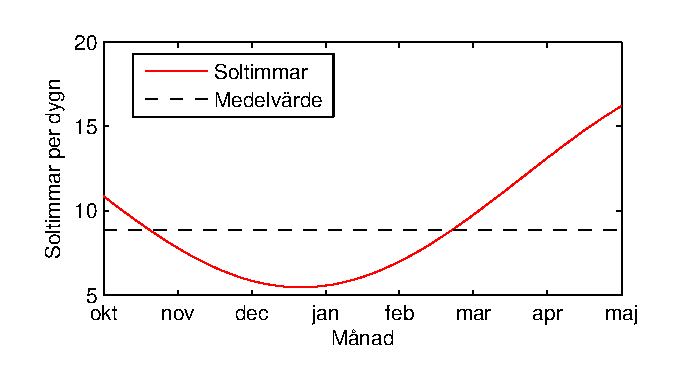
\includegraphics{images/sunhours.eps}
\caption{Antal timmar i ett dygn då solen är ovanför horisonten beräknat för månaderna under eldningsperioden.
Här är medelvärdet markerat med en streckad linje. Medelvärdet har beräknats vara
$\bar{\tau}=\unit[9,39]{~timmar~per~dygn}$.}
\label{fig:sunhours}
\end{figure}

\noindent
För att estimera hur mycket energi som det går att spara på att ta hänsyn till solen kommer arbetet
senare att behandla en decemberdag. Denna dag har sedan behandlats med antagandet att den är solig samt
med antagandet att den är molning. Vi benämner energiåtgången för den molniga dagen som $Q_H$ och
$Q_L$ som energiåtgången den soliga dagen. Värden på dessa kommer sedan att användas tillsammans med
ovanstående beräkningar för att estimera totala mängden energi som det går att spara. 

Från SMHIs väderstatistik går det att utläsa att $\unit[8]{\%}$ av eldningsperiodens timmar är soliga.\cite{SMHIdata}
Detta motsvarar då $\unit[1,92]{~soliga~timmar}$ i snitt per dygn. Härnäst betecknas andelen timmar som är molniga som
$p = 1,92/9,32 = \unit[20,45]{\%}$. Nu beräknas medelenergiåtgången per dygn $Q$ enligt

\begin{equation}
Q = pQ_H + (1-p)Q_L
\end{equation}

\noindent
Slutligen kan kvoten $Q/Q_H$ beräknas vilket ger ett uttryck för hur mycket energi det går att spara

\begin{equation}
\frac{Q}{Q_H} = \frac{pQ_H + (1-p)Q_L}{Q_H} = p+(1-p)\frac{Q_L}{Q_H}
\end{equation}

\subsection{Solinstrålning}
För att beräkna den totala effekt solstrålning tillför byggnaden behövs fönstrenas vinkelberoende g-värden, presenterat i avsnitt \ref{gvalue}, och för att bestämma detta värde ur \eqref{eq:radiationwindowstheory:gvalue} behöver parametern $z = \theta/90$ beräknas, där $\theta$ är vinkeln mellan solstrålingens riktning och fönstrets normal i grader. Detta kan göras genom att utgå från aktuellt datum och tid på dygnet.

En metod för att räkna ut solens position presenteras i \cite{walraven78} och en Matlabfunktion baserad på samma artikel kan ses i appendix \ref{app:sunposition}. Argumenten i denna funktion består av longitudinella och latitudinella koordinater för aktuella platsen samt datum och tidpunkt. För Walleriusgatan är koordinaterna ungefär $\unit[12]{^\circ}$ E respektive $\unit[58]{^\circ}$ N.

När azimuthala och altitudinella vinklarna, det vill säga $\beta$ respektive $\alpha$, relativt ett väderstreck respektive horisonten har beräknats relateras infallsvinkeln mot glaset, $\theta$, som

\begin{equation} 
\theta = \arccos{\left( \cos{\left(\beta - \gamma\right)}\cos{\left(\alpha\right)}\right)}
\end{equation}

där $\gamma$ är vinkeln mellan fönstrets normal och väderstrecket mot vilken azimuthala vinkeln anges. Detta görs med funktionen angletheta i appendix \ref{app:sunwindows}.

Med dessa samband tillgängliga kan effektflödet på grund av solstrålning genom fönster beräknas, vilket kan göras med funktionerna \textit{gvalue} samt \textit{effekt} från appendix \ref{app:sunwindows}. Nödvändiga argument för dessa funktioner är g-värdet vid vinkelrätt infallande strålning samt konstanterna p och q från \eqref{eq:gconstants}. % Repetera ekvationen?

För att ge ett exempel på hur effekten varierar med solintensiteten måste en approximativ funktion byggas upp som beskriver solens intensitet vid marknivå som funktion av vinkeln över horisonten. Om vi antar att intensiteten är $I_o = \unit[1370]{Wm^-2}$ utanför atmosfären kan detta beskrivas med ett exponentiellt samband, $I = I_oe^{-\mu x}$ där $\mu$ kallas för atmosfärens absorbtionskoefficient som sätts till $mu\approx \unit[4.6\cdot 10^{-5}]{m^{-1}}$ och x är atmosfärens tjocklek mellan betraktaren och solen, i meter. Atmosfären antas dessutom vara som en homogen heltäckande sfär runt jorden och ungefär $\unit[15]{km}$ tjock vertikalt uppåt överallt på jordens yta. x kan nu beskrivas med solens höjd över horisonten, och ges av

\begin{equation}
x = R\cos{90+\alpha} + \sqrt{\left(R\cos{90+\alpha}\right)^2 + \left( R+15\right)^2 - R^2}
\end{equation}

där $\alpha$ är vinkeln mellan horisonten och solen och $R\approx\unit[6,731\cdot 10^3]{m}$ betecknar jordens radie \cite{physicshandbook}. Detta följer från cosinussatsen. % Källa på siffran mu?

\subsection{Inverkan av skuggor, rummets interiör och dylikt}

Sambanden ovan gäller då all strålning som passerar rutan stannar i rummet. Svårigheter uppstår när exempelvis persienner används. Dessutom har ingen hänsyn tagits till det faktum att omkringliggande byggnader kommer att blockera den direkta solstrålningen vid vissa tidpunkter.

Hur mycket av solinstrålningen som blockeras av persienner och gardiner är oerhört svårt att räkna ut. För det första hyser den parametern ett vinkelberoende, det vill säga beroende på persiennens konfiguration, färg och vinkel kommer olika mycket att reflekteras tillbaka ut ur fönstret. För det andra måste hänsyn tas till mänskliga faktorer. Naturligtvis kommer vinkeln på persiennen att förändras vid godtyckliga tidpunkter. För att modellera sådana anordningar kan man enligt \cite{ASHRAE09} lägga till en vinkelberoende faktor, $0 \le R_{ref}\left( \theta \right) \le 1$, i \eqref{eq:totalsun} så att den slutliga formeln för solinstrålning genom fönster blir


\begin{equation}\label{eq:totalsunblinds}
Q = R_{ref}\left( \theta \right) \cdot g\left( \theta \right) \cdot A \cdot I_0 \cos{\theta} \unit[]{W}.
\end{equation}

Vid exempelberäkningarna i nästa avsnitt har dock ingen hänsyn tagits till denna koefficient, som satts konstant $R_{ref}$.

Effekten av skuggorna som orsakas av grannbyggnader i området kan också tas med i beräkningarna genom att mäta geometrin på omgivande byggnader, men detta är ett tidsödande moment och görs inte i denna rapport.

\subsection{Långvågsstrålning}\label{subsec:IRmethod}

Vid beräkning av energiflödet på grund av långvågig strålning antas att luften precis innanför fönstret håller konstant temperatur, $\unit[20]{^{\circ}C}$ och att de ''synliga'' ytorna utanför fönstret håller en temperatur motsvarande utomhustemperaturen, $T_{ute}$. Enligt beräkningen i avsnitt \ref{IR} kommer 75\% av den incidenta strålningen passera ett treglasfönster. Med detta i åtanke leder Stefan-Boltzmanns lag, \eqref{eq:boltzmanslag}, till, om det antas stråla som en svartkropp, att $q_{IR} = 0,75 \cdot \sigma \unit[\left( 293^4 - T_{ute}^4\right)]{Wm^{-2}}$. Den totala effekt som flödar ut på grund av svartkroppsstrålning blir då $\unit[q_{IR}\cdot A]{W}$, där $A$ är totala arean av fönsterglas på byggnaden.

\subsection{Övriga strålningseffekter}

Då solen skiner kommer en viss andel direkt solstrålning att reflekteras från omgivande byggnader, växtlighet och dylikt för att sedan öka på intesiteten mot fönsterrutorna. Eftersom en andel av den direkt infallande solstrålningen genom fönsterrutorna även kommer att reflekteras mot rummens interiör och stråla ut igen har vi valt att inte ta hänsyn till dessa flöden, som beror starkt på omgivningens respektive interiörens utformning.

